\section{Kế hoạch làm việc}

\subsection{Nhiệm vụ}

Với phạm vi của môn học KNCN, các công việc cần thực hiện được xác định bao gồm một chuỗi các giai đoạn quan trọng nhằm đảm bảo quá trình xây dựng website anime diễn ra hiệu quả và theo đúng kế hoạch:

\textbf{Bước 1: Thu thập thông tin và yêu cầu về website} \\
Đây là bước đầu tiên và đóng vai trò quan trọng trong việc xác định mục tiêu và chức năng của website anime.
\begin{itemize}
    \item Tìm hiểu nhu cầu của người dùng,
    \item Phân tích các yêu cầu chức năng cũng như phi chức năng cần thiết.
\end{itemize}
Hiện tại, quá trình này gần như đã hoàn thành, cung cấp nền tảng vững chắc để bước vào các giai đoạn tiếp theo.

\textbf{Bước 2: Xây dựng bản thiết kế của trang web}
\begin{itemize}
    \item \textbf{Thiết kế giao diện}: Sử dụng công cụ Figma, nhóm sẽ thiết kế các yếu tố giao diện người dùng (UI) của website. Bản thiết kế này sẽ bao gồm các trang chính như:
    \begin{itemize}
        \item Trang chủ,
        \item Trang chi tiết anime,
        \item Trang phát sóng tập phim,
        \item Trang đăng nhập/đăng ký, 
        \item Các trang phụ khác.
    \end{itemize}
    Figma cho phép nhóm dễ dàng chỉnh sửa, xem xét và chia sẻ bản thiết kế để nhận phản hồi.
    
    \item \textbf{Thiết kế cơ sở dữ liệu (CSDL)}: Do giới hạn về thời gian và nguồn lực, việc thiết kế CSDL hoàn chỉnh như trong thực tế sẽ không khả thi. Vì vậy, nhóm sẽ:
    \begin{itemize}
        \item Thiết kế một CSDL mẫu đáp ứng các yêu cầu chính của hệ thống,
        \item Sử dụng API và dữ liệu có sẵn cho việc demo.
    \end{itemize}
\end{itemize}

\textbf{Bước 3: Hiện thực trang web} \\
Sau khi hoàn tất giai đoạn thiết kế, nhóm sẽ thực hiện:
\begin{itemize}
    \item Phát triển mã nguồn của website anime,
    \item Tích hợp với API để lấy dữ liệu,
    \item Đảm bảo các chức năng hoạt động như mong đợi,
    \item Xem xét các khía cạnh quan trọng như hiệu suất, khả năng tương thích trên nhiều thiết bị, và tính bảo mật.
\end{itemize}

\textbf{Bước 4: Demo thiết kế và kiểm thử} \\
Nhóm sẽ tiến hành:
\begin{itemize}
    \item Demo trang web để kiểm tra tính khả dụng, giao diện và trải nghiệm người dùng,
    \item Kiểm thử chức năng, hiệu suất, và tính tương thích trên các trình duyệt và thiết bị khác nhau,
    \item Tổng hợp phản hồi, chỉnh sửa và hoàn thiện website để đạt được chất lượng tốt nhất.
\end{itemize}

$\Rightarrow$ Kế hoạch này giúp nhóm tiếp cận từng giai đoạn một cách có hệ thống, đảm bảo việc xây dựng website anime được thực hiện hiệu quả và đáp ứng được yêu cầu của môn học KNCN.

\subsection{Phân công}

\textbf{Tuần 1}: 26/08/2024 - 01/09/2024

Trong tuần đầu tiên, các thành viên sẽ có buổi gặp mặt ban đầu để hình thành nhóm làm việc. Sau khi nhóm được lập, để duy trì liên lạc, nhóm sẽ tạo kênh trao đổi trên các nền tảng như Zalo, Facebook. Đây sẽ là nơi nhóm thường xuyên cập nhật tiến độ, thảo luận các vấn đề trực tuyến, giúp đảm bảo sự phối hợp linh hoạt và hiệu quả ngay cả khi không thể gặp trực tiếp.
\vspace{1cm}
\\
\textbf{Tuần 2}: 02/09/2024 - 08/09/2024

\textbf{Ngày họp:} 04/09/2024 \\
Trong tuần đầu tiên, nhóm sẽ thực hiện các công việc khởi đầu dự án, bao gồm:
\begin{itemize}
    \item \textbf{Thu thập yêu cầu}: Thực hiện khảo sát và phân tích nhu cầu từ người dùng tiềm năng, xác định các tính năng quan trọng và trải nghiệm mà website cần cung cấp.
    \item \textbf{Tổng hợp tài liệu yêu cầu}: Tất cả các yêu cầu sẽ được tổng hợp lại thành một tài liệu chi tiết, là cơ sở để định hướng cho các bước phát triển tiếp theo.
\end{itemize}
\vspace{1cm}
\textbf{Tuần 3}: 09/09/2024 - 15/09/2024

\textbf{Ngày họp:} 10/09/2024 \\
Trong tuần này, nhóm sẽ tiến hành họp để thảo luận và đưa ra quyết định về các công nghệ sẽ sử dụng trong quá trình phát triển trang web. Cụ thể, các hoạt động bao gồm:
\begin{itemize}
    \item \textbf{Phân tích ưu và nhược điểm}: Đánh giá các công nghệ dựa trên tính khả thi, hiệu suất, và khả năng tích hợp.
    \begin{itemize}
        \item Ngôn ngữ lập trình: Typescript;
        \item Framework phát triển web: NextJS;
        \item Cơ sở dữ liệu: MongoDB;
        \item Object-Relational Mapping: Prisma;
        \item Các công cụ hỗ trợ phát triển: Git, Docker.
    \end{itemize}
    \item \textbf{Quyết định công nghệ sử dụng}: Dựa trên buổi họp, nhóm sẽ thống nhất về công nghệ phù hợp nhất với yêu cầu dự án.
\end{itemize}
\textbf{11/09/2024 - 17/09/2024:} Vinh Hiển thiết kế giao diện (figma) cho 3 trang chính của website: Trang chủ, Trang chi tiết anime, Trang xem anime theo tập. \href{https://www.figma.com/design/J4VbkPcCrv7e07qyR7bimC/Anime-Web---Professional-Skills-for-Engineer-Assignment?node-id=0-1\&t=3CpS6XH3ANF1a3Fo-0}{Bản thiết kế figma}
\\
\begin{figure}[H]
    \centering
    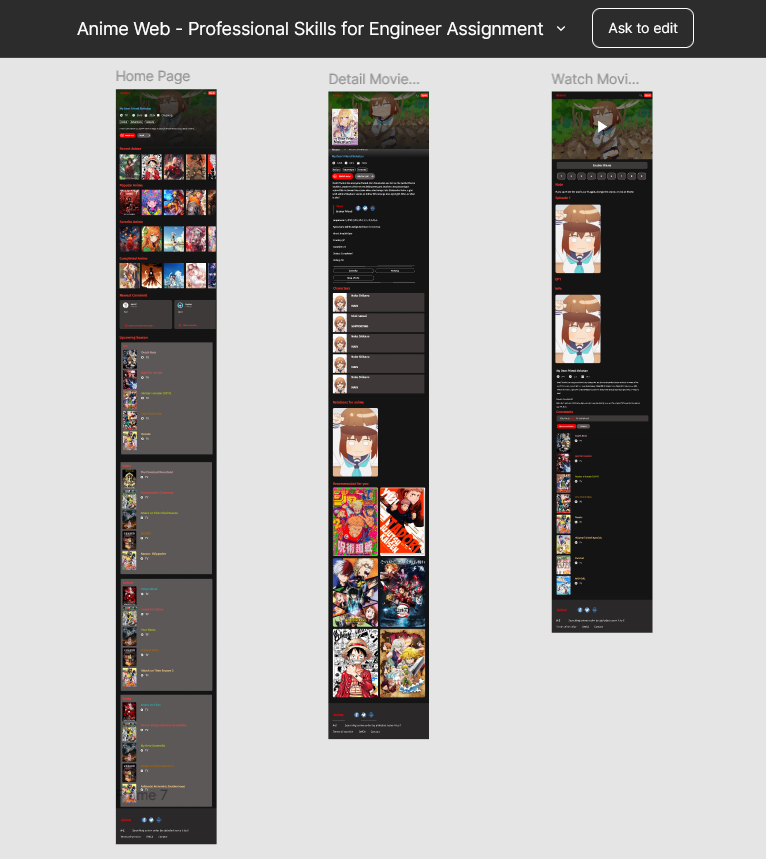
\includegraphics[width=0.5\linewidth]{content/planning/image/figma.png}
    \caption{Preview design}
    \label{fig:enter-label}
\end{figure}

\textbf{11/09/2024 - 17/09/2024:} Trí Hùng khởi tạo mã nguồn (Database, API, Đăng nhập/ Đăng ký). \href{https://github.com/hungdt31/next-anime-kncn}{https://github.com/hungdt31/next-anime-kncn}
\vspace{1cm}
\\
\textbf{Tuần 4}: 16/09/2024 - 22/09/2024

\textbf{18/09/2024 - 22/09/2024:} Trí Hùng code Trang chủ. \\
\begin{figure}[H]
    \centering
    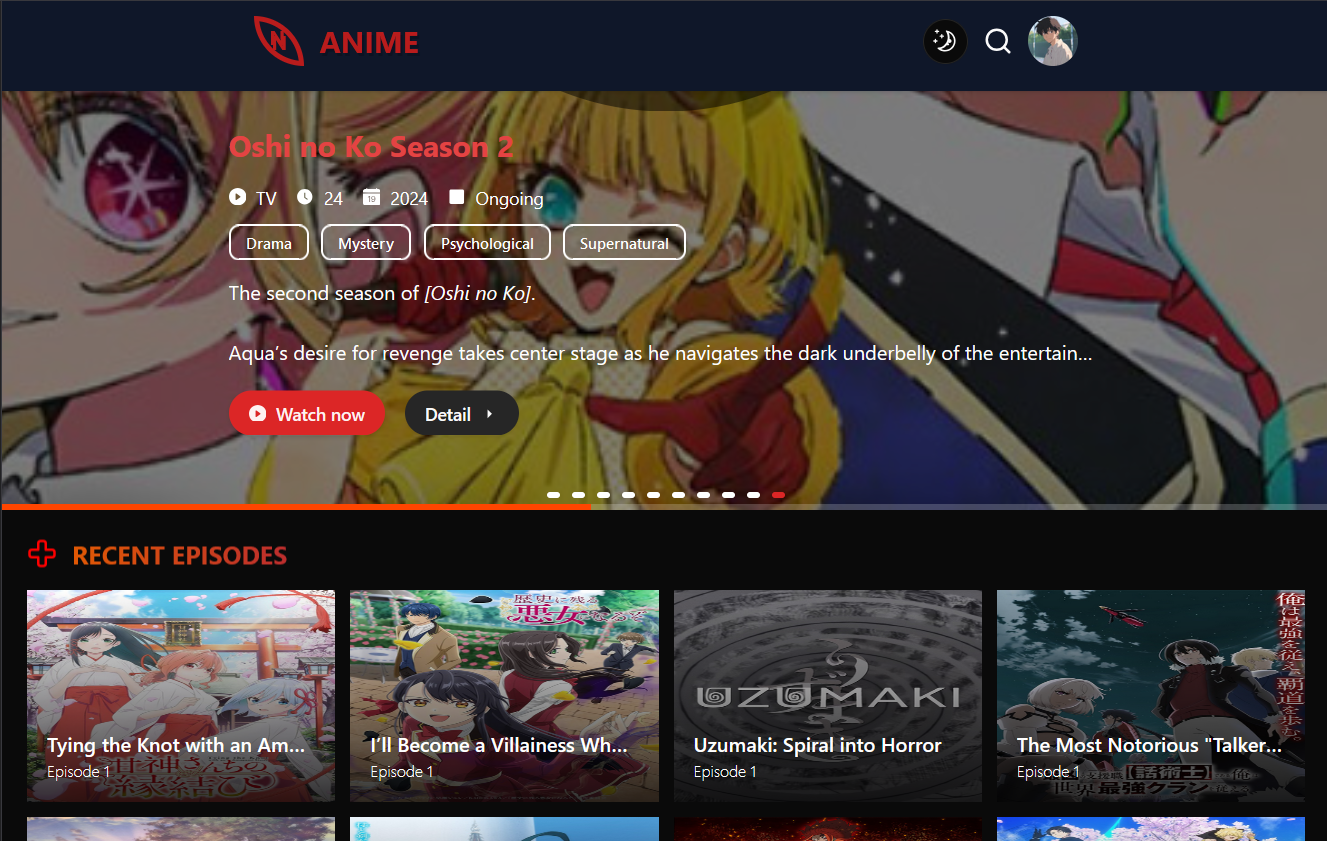
\includegraphics[width=0.8\linewidth]{content/planning/image/home.png}
    \caption{Home Page Preview}
    \label{fig:enter-label}
\end{figure}
\textbf{18/09/2024 - 22/09/2024:} Hoàng Hùng code Trang xem anime theo tập.\\
\begin{figure}[H]
    \centering
    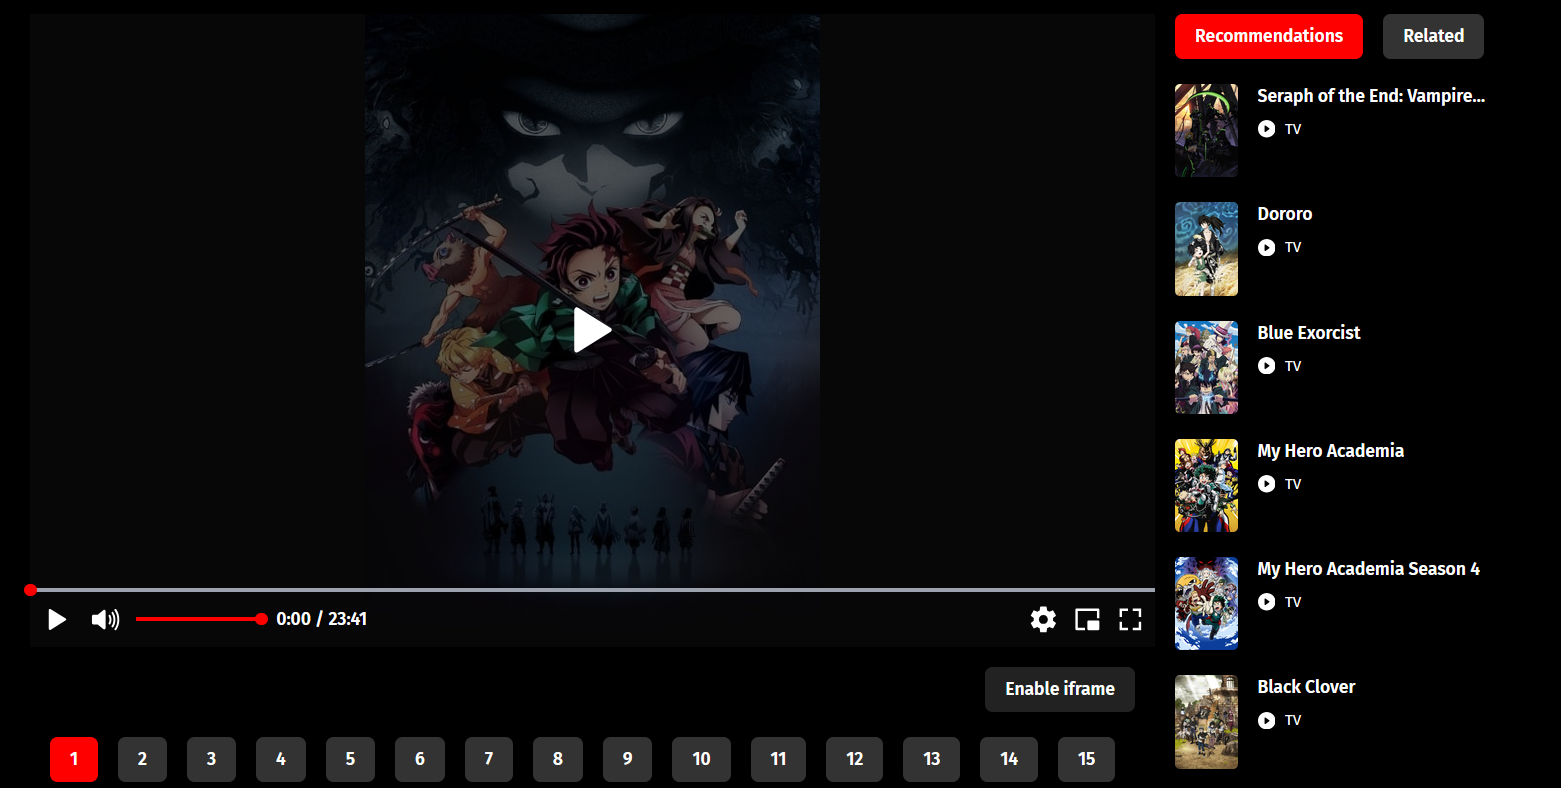
\includegraphics[width=0.8\linewidth]{content/planning/image/watch.png}
    \caption{Watch Anime Preview}
    \label{fig:enter-label}
\end{figure}
\textbf{18/09/2024 - 22/09/2024:} Thanh Điền code Trang chi tiết anime. \\
\begin{figure}[H]
    \centering
    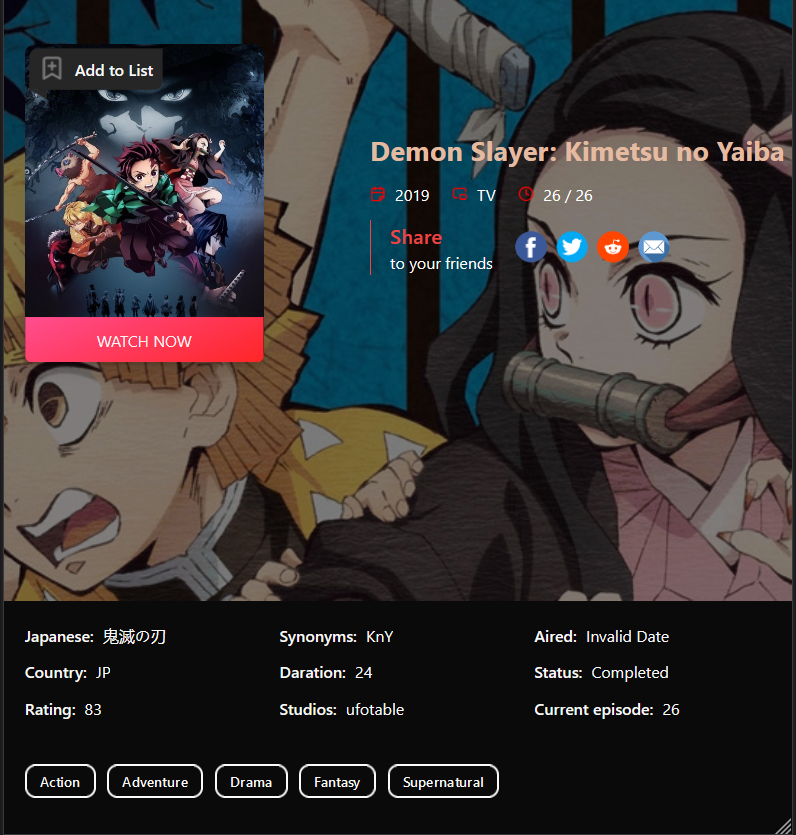
\includegraphics[width=0.6\linewidth]{content/planning/image/detail.png}
    \caption{Detail Anime Preview}
    \label{fig:enter-label}
\end{figure}

\textbf{Tuần 5}: 23/09/2024 - 29/09/2024

\textbf{23/09/2024 - 27/09/2024:} Đăng Bách viết báo cáo nội dung công việc.\\
\textbf{28/09/2024 - 29/09/2024:} Trí Hùng và Thanh Điền kiểm tra và chỉnh sửa nội dung, hoàn thành báo cáo. 
\vspace{1cm}
\\
\textbf{Tuần 6}: 30/09/2024 - 06/10/2024

\textbf{30/09/2024 - 03/10/2024:} Đăng Bách chuyển đổi báo cáo sang bài thuyết trình. \\
\textbf{04/09/2024:} Thuyết trình đợt 1.
\pagebreak